%\setchapterstyle{kao}
\setchapterpreamble[u]{\margintoc}
\chapter{第一讲:平行四边形的性质}
%\labch{pingxing}

\section{轴对称与中心对称}
八上部分,我们已经学习了两大对称图形中的一种 --- 轴对称图形。简单说,轴对称图形就是沿着一条直线翻折后,
直线两边的部分能够完全重合的图形,建立在全等、垂直平分线的基础上,我们
可以很容易的发现轴对称图形的性质:\underline{\textbf{\textit{一轴二点垂直等距}}}:


\begin{itemize}
    \item “一轴二点”:对称轴和对称轴两侧的对应点
    \item “等距”:对应点到对称轴的距离相等
    \item “垂直”:对应点的连线垂直于对称轴
\end{itemize}


基于这样的“性质”,我们就可以发展出对轴对称图形的“判定”。


% 轴对称图形判定图
\tikzset{every picture/.style={line width=0.75pt}} %set default line width to 0.75pt        
\begin{tikzpicture}[x=0.75pt,y=0.75pt,yscale=-1,xscale=1]
%uncomment if require: \path (0,1237); %set diagram left start at 0, and has height of 1237
%Shape: Trapezoid [id:dp29138151141672464] 
\draw   (533,1101.4) -- (547.94,1051.61) -- (607.4,1051.61) -- (622.33,1101.4) -- cycle ;
%Straight Lines [id:da17552131169444474] 
\draw  [dash pattern={on 1.5pt off 2.25pt}]  (578.56,1019.49) -- (578.56,1138.33) ;
%Curve Lines [id:da7998947700195351] 
\draw  [dash pattern={on 3.75pt off 3pt on 7.5pt off 1.5pt}]  (549.62,1051.61) .. controls (584.63,1028) and (578.81,1033.7) .. (604.13,1050.56) ;
\draw [shift={(605.72,1051.61)}, rotate = 213.04] [color={rgb, 255:red, 0; green, 0; blue, 0 }  ][line width=0.75]    (10.93,-3.29) .. controls (6.95,-1.4) and (3.31,-0.3) .. (0,0) .. controls (3.31,0.3) and (6.95,1.4) .. (10.93,3.29)   ;
\draw [shift={(549.62,1051.61)}, rotate = 326.01] [color={rgb, 255:red, 0; green, 0; blue, 0 }  ][fill={rgb, 255:red, 0; green, 0; blue, 0 }  ][line width=0.75]      (0, 0) circle [x radius= 3.35, y radius= 3.35]   ;
%Curve Lines [id:da8905696886777257] 
\draw  [dash pattern={on 3.75pt off 3pt on 7.5pt off 1.5pt}]  (533,1101.4) .. controls (569.96,1122.75) and (586.11,1125.41) .. (620.74,1102.46) ;
\draw [shift={(622.33,1101.4)}, rotate = 146.01] [color={rgb, 255:red, 0; green, 0; blue, 0 }  ][line width=0.75]    (10.93,-3.29) .. controls (6.95,-1.4) and (3.31,-0.3) .. (0,0) .. controls (3.31,0.3) and (6.95,1.4) .. (10.93,3.29)   ;
\draw [shift={(533,1101.4)}, rotate = 30.02] [color={rgb, 255:red, 0; green, 0; blue, 0 }  ][fill={rgb, 255:red, 0; green, 0; blue, 0 }  ][line width=0.75]      (0, 0) circle [x radius= 3.35, y radius= 3.35]   ;
%Rounded Rect [id:dp26739840735837195] 
\draw   (278,1046.13) .. controls (278,1041.54) and (281.72,1037.82) .. (286.3,1037.82) -- (332.28,1037.82) .. controls (336.87,1037.82) and (340.59,1041.54) .. (340.59,1046.13) -- (340.59,1071.03) .. controls (340.59,1075.62) and (336.87,1079.34) .. (332.28,1079.34) -- (286.3,1079.34) .. controls (281.72,1079.34) and (278,1075.62) .. (278,1071.03) -- cycle ;
%Rounded Rect [id:dp9918082181524119] 
\draw   (406.75,1046.13) .. controls (406.75,1041.54) and (410.46,1037.82) .. (415.05,1037.82) -- (461.03,1037.82) .. controls (465.62,1037.82) and (469.33,1041.54) .. (469.33,1046.13) -- (469.33,1071.03) .. controls (469.33,1075.62) and (465.62,1079.34) .. (461.03,1079.34) -- (415.05,1079.34) .. controls (410.46,1079.34) and (406.75,1075.62) .. (406.75,1071.03) -- cycle ;
%Straight Lines [id:da8877758210692699] 
\draw    (339.69,1057.12) -- (405.94,1057.12) ;
\draw [shift={(407.94,1057.12)}, rotate = 180] [color={rgb, 255:red, 0; green, 0; blue, 0 }  ][line width=0.75]    (10.93,-3.29) .. controls (6.95,-1.4) and (3.31,-0.3) .. (0,0) .. controls (3.31,0.3) and (6.95,1.4) .. (10.93,3.29)   ;
%Curve Lines [id:da10896623380423431] 
\draw    (438.34,1079.17) .. controls (444.53,1137.39) and (307.9,1140.68) .. (308.63,1083.68) ;
\draw [shift={(308.7,1081.93)}, rotate = 93.48] [color={rgb, 255:red, 0; green, 0; blue, 0 }  ][line width=0.75]    (10.93,-3.29) .. controls (6.95,-1.4) and (3.31,-0.3) .. (0,0) .. controls (3.31,0.3) and (6.95,1.4) .. (10.93,3.29)   ;
% Text Node
\draw (309.29,1058.58) node  [font=\scriptsize] [align=left] {图形上的点};
% Text Node
\draw (438.04,1058.58) node  [font=\scriptsize] [align=left] {对应点};
% Text Node
\draw (344.67,1039.93) node [anchor=north west][inner sep=0.75pt]  [font=\scriptsize] [align=left] {过对称轴做};
% Text Node
\draw (330.51,1101.5) node [anchor=north west][inner sep=0.75pt]  [font=\scriptsize] [align=left] {对应点仍在原图上};
\end{tikzpicture}

由上面的分析,判断一个图形是否 “轴对称” 图形的关键是,\\\underline{\textbf{\textit{对应点是否在原图上}}}
。我们借由这一判定规则发现等腰三角形、正方形、矩形,都是轴对称图形。当然,自然界还有一种
对称 --- “中心对称”!顾名思义,这个图形不是关于一个轴,而是关于一个中心点对称。

\begin{marginfigure}
    \includegraphics[width=0.5\textwidth]{images/original_pointsymmetry14.png}
    \caption{扑克牌中的中心对称}
\end{marginfigure}





\tikzset{every picture/.style={line width=0.75pt}} %set default line width to 0.75pt        
\begin{tikzpicture}[x=0.75pt,y=0.75pt,yscale=-1,xscale=1]
%uncomment if require: \path (0,1741); %set diagram left start at 0, and has height of 1741
%Straight Lines [id:da18984128848065107] 
\draw    (554.33,1259.01) -- (617.33,1176.01) ;
%Curve Lines [id:da7684463427358112] 
\draw    (554.33,1259.01) .. controls (560.33,1205.01) and (612.33,1228.01) .. (617.33,1176.01) ;
\draw [shift={(617.33,1176.01)}, rotate = 275.49] [color={rgb, 255:red, 0; green, 0; blue, 0 }  ][fill={rgb, 255:red, 0; green, 0; blue, 0 }  ][line width=0.75]      (0, 0) circle [x radius= 3.35, y radius= 3.35]   ;
%Shape: Circle [id:dp41832069902269] 
\draw  [dash pattern={on 3.75pt off 3pt on 7.5pt off 1.5pt}] (584.17,1215.84) .. controls (584.17,1213.82) and (585.81,1212.18) .. (587.83,1212.18) .. controls (589.86,1212.18) and (591.5,1213.82) .. (591.5,1215.84) .. controls (591.5,1217.87) and (589.86,1219.51) .. (587.83,1219.51) .. controls (585.81,1219.51) and (584.17,1217.87) .. (584.17,1215.84) -- cycle ;
%Curve Lines [id:da7768213142838352] 
\draw  [dash pattern={on 3.75pt off 3pt on 7.5pt off 1.5pt}]  (614.99,1175.54) .. controls (610.21,1174.62) and (605.64,1173.97) .. (601.28,1173.57) .. controls (542.07,1168.12) and (521.25,1208.93) .. (549.46,1252.68) ;
\draw [shift={(550.33,1254.01)}, rotate = 236.31] [color={rgb, 255:red, 0; green, 0; blue, 0 }  ][line width=0.75]    (10.93,-3.29) .. controls (6.95,-1.4) and (3.31,-0.3) .. (0,0) .. controls (3.31,0.3) and (6.95,1.4) .. (10.93,3.29)   ;
\draw [shift={(617.33,1176.01)}, rotate = 191.77] [color={rgb, 255:red, 0; green, 0; blue, 0 }  ][line width=0.75]      (0, 0) circle [x radius= 3.35, y radius= 3.35]   ;
%Rounded Rect [id:dp9719046231895392] 
\draw   (279,1178.13) .. controls (279,1173.54) and (282.72,1169.82) .. (287.3,1169.82) -- (333.28,1169.82) .. controls (337.87,1169.82) and (341.59,1173.54) .. (341.59,1178.13) -- (341.59,1203.03) .. controls (341.59,1207.62) and (337.87,1211.34) .. (333.28,1211.34) -- (287.3,1211.34) .. controls (282.72,1211.34) and (279,1207.62) .. (279,1203.03) -- cycle ;
%Rounded Rect [id:dp7904907205889073] 
\draw   (407.75,1178.13) .. controls (407.75,1173.54) and (411.46,1169.82) .. (416.05,1169.82) -- (462.03,1169.82) .. controls (466.62,1169.82) and (470.33,1173.54) .. (470.33,1178.13) -- (470.33,1203.03) .. controls (470.33,1207.62) and (466.62,1211.34) .. (462.03,1211.34) -- (416.05,1211.34) .. controls (411.46,1211.34) and (407.75,1207.62) .. (407.75,1203.03) -- cycle ;
%Straight Lines [id:da6428118451084119] 
\draw    (340.69,1189.12) -- (406.94,1189.12) ;
\draw [shift={(408.94,1189.12)}, rotate = 180] [color={rgb, 255:red, 0; green, 0; blue, 0 }  ][line width=0.75]    (10.93,-3.29) .. controls (6.95,-1.4) and (3.31,-0.3) .. (0,0) .. controls (3.31,0.3) and (6.95,1.4) .. (10.93,3.29)   ;
%Curve Lines [id:da015808274443750436] 
\draw    (439.34,1211.17) .. controls (445.53,1269.39) and (308.9,1272.68) .. (309.63,1215.68) ;
\draw [shift={(309.7,1213.93)}, rotate = 93.48] [color={rgb, 255:red, 0; green, 0; blue, 0 }  ][line width=0.75]    (10.93,-3.29) .. controls (6.95,-1.4) and (3.31,-0.3) .. (0,0) .. controls (3.31,0.3) and (6.95,1.4) .. (10.93,3.29)   ;
% Text Node
\draw (310.29,1190.58) node  [font=\scriptsize] [align=left] {图形上的点};
% Text Node
\draw (439.04,1190.58) node  [font=\scriptsize] [align=left] {对应点};
% Text Node
\draw (340.67,1171.93) node [anchor=north west][inner sep=0.75pt]  [font=\scriptsize] [align=left] {过对称中心做};
% Text Node
\draw (331.51,1233.5) node [anchor=north west][inner sep=0.75pt]  [font=\scriptsize] [align=left] {对应点仍在原图上};
\end{tikzpicture}

\begin{definition}
    \ubi{轴对称图形}:图形上任意一点,关于对称轴的对应点(等效于沿对称轴翻折)在原图上。
\end{definition}

\begin{definition}
    \ubi{中心对称图形}:图形上任意一点,关于对称中心的对应点(等效于旋转$180^o$)在原图上。    
\end{definition}


\clearpage

\example{“翻折” 产生 “轴对称”;“旋转” 产生 “中心对称”!不论轴对称还是中心对称,在数学和物理中都有着广泛的应用,
比如下面四个函数图像。观察图像,识别抽对称或中心对称。}

\marginnote{
    \tikzset{every picture/.style={line width=0.75pt}} %set default line width to 0.75pt        
    \begin{tikzpicture}[x=0.75pt,y=0.75pt,yscale=-1,xscale=1]
    %uncomment if require: \path (0,361); %set diagram left start at 0, and has height of 361
    %Straight Lines [id:da439573922876374] 
    \draw    (87,218) -- (87,247.14) ;
    %Straight Lines [id:da5676159915309784] 
    \draw    (87,247.14) -- (105,247.14) ;
    %Straight Lines [id:da32984765214506484] 
    \draw    (87,247) -- (87,276.14) ;
    %Straight Lines [id:da33250566801593395] 
    \draw    (87,276.14) -- (105,276.14) ;
    % Text Node
    \draw (65,200) node [anchor=north west][inner sep=0.75pt]  [font=\scriptsize] [align=left] {看图技巧:对应点是否在原图上};
    % Text Node
    \draw (108,238) node [anchor=north west][inner sep=0.75pt]  [font=\scriptsize] [align=left] {关于线对称};
    % Text Node
    \draw (109,266) node [anchor=north west][inner sep=0.75pt]  [font=\scriptsize] [align=left] {关于点对称};
    \end{tikzpicture}
}




\marginnote{
    \tikzset{every picture/.style={line width=0.75pt}} %set default line width to 0.75pt        
    \begin{tikzpicture}[x=0.75pt,y=0.75pt,yscale=-1,xscale=1]
    %uncomment if require: \path (0,361); %set diagram left start at 0, and has height of 361
    %Straight Lines [id:da439573922876374] 
    \draw    (87,218) -- (87,247.14) ;
    %Straight Lines [id:da5676159915309784] 
    \draw    (87,247.14) -- (105,247.14) ;
    %Straight Lines [id:da32984765214506484] 
    \draw    (87,247) -- (87,276.14) ;
    %Straight Lines [id:da33250566801593395] 
    \draw    (87,276.14) -- (105,276.14) ;
    % Text Node
    \draw (65,200) node [anchor=north west][inner sep=0.75pt]  [font=\scriptsize] [align=left] {对应点是否在原图上};
    % Text Node
    \draw (108,238) node [anchor=north west][inner sep=0.75pt]  [font=\scriptsize] [align=left] {关于线对称};
    % Text Node
    \draw (109,266) node [anchor=north west][inner sep=0.75pt]  [font=\scriptsize] [align=left] {关于点对称};
    \end{tikzpicture}
}

% 4 个函数图像
\tikzset{every picture/.style={line width=0.75pt}} %set default line width to 0.75pt        
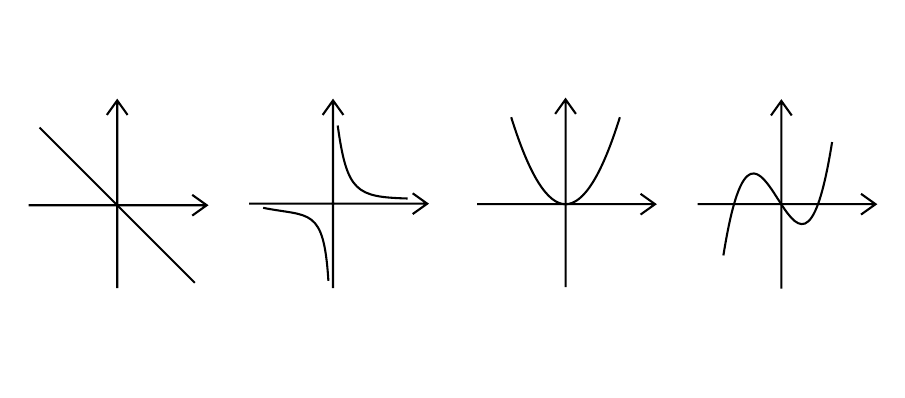
\begin{tikzpicture}[x=0.75pt,y=0.75pt,yscale=-1,xscale=1]
%uncomment if require: \path (0,1485); %set diagram left start at 0, and has height of 1485
%Shape: Axis 2D [id:dp012732840762755826] 
\draw  (272.33,1320.27) -- (358.11,1320.27)(314.97,1269.77) -- (314.97,1360.17) (351.11,1315.27) -- (358.11,1320.27) -- (351.11,1325.27) (309.97,1276.77) -- (314.97,1269.77) -- (319.97,1276.77)  ;
%Shape: Parabola [id:dp1092507051161018] 
\draw   (288.79,1278.38) .. controls (306.25,1334.24) and (323.7,1334.24) .. (341.15,1278.38) ;
%Shape: Axis 2D [id:dp4872769877228149] 
\draw  (378.56,1320.27) -- (464.33,1320.27)(418.95,1270.52) -- (418.95,1360.92) (457.33,1315.27) -- (464.33,1320.27) -- (457.33,1325.27) (413.95,1277.52) -- (418.95,1270.52) -- (423.95,1277.52)  ;
%Shape: Polynomial [id:dp41529725511086] 
\draw   (391.02,1344.96) .. controls (408.48,1235.74) and (425.93,1399.57) .. (443.39,1290.35) ;
%Shape: Axis 2D [id:dp6057578400327135] 
\draw  (56.33,1320.77) -- (142.11,1320.77)(98.97,1270.27) -- (98.97,1360.67) (135.11,1315.77) -- (142.11,1320.77) -- (135.11,1325.77) (93.97,1277.27) -- (98.97,1270.27) -- (103.97,1277.27)  ;
%Straight Lines [id:da3784861620097686] 
\draw    (61.57,1283.37) -- (136.37,1358.17) ;
%Shape: Axis 2D [id:dp22548908292260683] 
\draw  (162.56,1320.02) -- (248.33,1320.02)(202.95,1270.27) -- (202.95,1360.67) (241.33,1315.02) -- (248.33,1320.02) -- (241.33,1325.02) (197.95,1277.27) -- (202.95,1270.27) -- (207.95,1277.27)  ;
%Curve Lines [id:da06487889473093755] 
\draw    (205.2,1282.37) .. controls (209.68,1314.54) and (214.17,1316.78) .. (238.86,1317.53) ;
%Curve Lines [id:da25453125841321866] 
\draw    (169.29,1322.02) .. controls (191.73,1326.51) and (198.46,1321.27) .. (200.71,1357.18) ;
\end{tikzpicture}

\vspace{1cm}

%TODO
\begin{marginfigure}
    \includegraphics[width=0.4\textwidth]{1-5-6shape.jpg}
\end{marginfigure}

\begin{example}
    图中其中既是轴对称图形又是中心对称图形的是( \ \ )
    \includegraphics{1-t-symetry.jpg}
\end{example}

\marginnote{奇数边正多边形,轴对称;偶数边正多边形,轴对称+中心对称}

\vspace{2cm}



\section{绘制轴对称和中心对称图形}

\marginnote{
    \begin{enumerate}
        \item 第一步:确定对称轴或对称中心。
        \item 第二步:根据对称轴或对称中心绘制对应点。
        \item 第三步:连接对应点,完成对称图形。
    \end{enumerate}
}

%----------------------------------------------------------------------------------------
% 绘图,轴对称中心对称


\tikzset{every picture/.style={line width=0.75pt}} %set default line width to 0.75pt        
\begin{tikzpicture}[x=0.75pt,y=0.75pt,yscale=-1,xscale=1]
%uncomment if require: \path (0,862); %set diagram left start at 0, and has height of 862
%Straight Lines [id:da384414329408274] 
\draw  [dash pattern={on 0.84pt off 2.51pt}]  (406.44,198.9) -- (457,247.19) ;
%Straight Lines [id:da42621078052121275] 
\draw  [dash pattern={on 0.84pt off 2.51pt}]  (391,248.19) -- (472.44,197.9) ;
%Straight Lines [id:da6431453526633546] 
\draw    (323,55.03) -- (323,131.14) ;
%Straight Lines [id:da13890380942488578] 
\draw    (303.74,73.15) -- (289.7,117.94) ;
\draw [shift={(289,120.19)}, rotate = 107.39] [color={rgb, 255:red, 0; green, 0; blue, 0 }  ][line width=0.75]      (0, 0) circle [x radius= 3.35, y radius= 3.35]   ;
\draw [shift={(304.44,70.9)}, rotate = 107.39] [color={rgb, 255:red, 0; green, 0; blue, 0 }  ][line width=0.75]      (0, 0) circle [x radius= 3.35, y radius= 3.35]   ;
%Straight Lines [id:da7228626390374118] 
\draw    (430.5,54.03) -- (430.5,134.14) ;
%Straight Lines [id:da27471904877190423] 
\draw    (403.74,76.15) -- (389.7,120.94) ;
\draw [shift={(389,123.19)}, rotate = 107.39] [color={rgb, 255:red, 0; green, 0; blue, 0 }  ][line width=0.75]      (0, 0) circle [x radius= 3.35, y radius= 3.35]   ;
\draw [shift={(404.44,73.9)}, rotate = 107.39] [color={rgb, 255:red, 0; green, 0; blue, 0 }  ][line width=0.75]      (0, 0) circle [x radius= 3.35, y radius= 3.35]   ;
%Shape: Trapezoid [id:dp8768743421620964] 
\draw  [line width=0.75]  (514,121.19) -- (528.78,71.9) -- (582.22,71.9) -- (597,121.19) -- cycle ;
%Straight Lines [id:da5898992052150023] 
\draw    (528.74,74.15) -- (514.7,118.94) ;
\draw [shift={(514,121.19)}, rotate = 107.39] [color={rgb, 255:red, 0; green, 0; blue, 0 }  ][line width=0.75]      (0, 0) circle [x radius= 3.35, y radius= 3.35]   ;
\draw [shift={(529.44,71.9)}, rotate = 107.39] [color={rgb, 255:red, 0; green, 0; blue, 0 }  ][line width=0.75]      (0, 0) circle [x radius= 3.35, y radius= 3.35]   ;
%Straight Lines [id:da20957961812073655] 
\draw    (582.92,74.15) -- (596.95,118.94) ;
\draw [shift={(597.65,121.19)}, rotate = 72.61] [color={rgb, 255:red, 0; green, 0; blue, 0 }  ][line width=0.75]      (0, 0) circle [x radius= 3.35, y radius= 3.35]   ;
\draw [shift={(582.22,71.9)}, rotate = 72.61] [color={rgb, 255:red, 0; green, 0; blue, 0 }  ][line width=0.75]      (0, 0) circle [x radius= 3.35, y radius= 3.35]   ;
%Straight Lines [id:da22146470569186172] 
\draw    (459.6,76.15) -- (473.63,120.94) ;
\draw [shift={(474.33,123.19)}, rotate = 72.61] [color={rgb, 255:red, 0; green, 0; blue, 0 }  ][line width=0.75]      (0, 0) circle [x radius= 3.35, y radius= 3.35]   ;
\draw [shift={(458.9,73.9)}, rotate = 72.61] [color={rgb, 255:red, 0; green, 0; blue, 0 }  ][line width=0.75]      (0, 0) circle [x radius= 3.35, y radius= 3.35]   ;
%Straight Lines [id:da4831815318450896] 
\draw  [dash pattern={on 0.84pt off 2.51pt}]  (404.44,73.9) -- (458.9,73.9) ;
%Straight Lines [id:da7099240975177683] 
\draw  [dash pattern={on 0.84pt off 2.51pt}]  (389,123.19) -- (474.33,123.19) ;
%Straight Lines [id:da8379561488619349] 
\draw    (312.74,203.15) -- (298.7,247.94) ;
\draw [shift={(298,250.19)}, rotate = 107.39] [color={rgb, 255:red, 0; green, 0; blue, 0 }  ][line width=0.75]      (0, 0) circle [x radius= 3.35, y radius= 3.35]   ;
\draw [shift={(313.44,200.9)}, rotate = 107.39] [color={rgb, 255:red, 0; green, 0; blue, 0 }  ][line width=0.75]      (0, 0) circle [x radius= 3.35, y radius= 3.35]   ;
%Shape: Circle [id:dp7795878187980079] 
\draw  [fill={rgb, 255:red, 0; green, 0; blue, 0 }  ,fill opacity=1 ] (336,226.17) .. controls (336,224.23) and (337.57,222.67) .. (339.5,222.67) .. controls (341.43,222.67) and (343,224.23) .. (343,226.17) .. controls (343,228.1) and (341.43,229.67) .. (339.5,229.67) .. controls (337.57,229.67) and (336,228.1) .. (336,226.17) -- cycle ;
%Straight Lines [id:da7829683688288385] 
\draw    (405.74,201.15) -- (391.7,245.94) ;
\draw [shift={(391,248.19)}, rotate = 107.39] [color={rgb, 255:red, 0; green, 0; blue, 0 }  ][line width=0.75]      (0, 0) circle [x radius= 3.35, y radius= 3.35]   ;
\draw [shift={(406.44,198.9)}, rotate = 107.39] [color={rgb, 255:red, 0; green, 0; blue, 0 }  ][line width=0.75]      (0, 0) circle [x radius= 3.35, y radius= 3.35]   ;
%Shape: Circle [id:dp35423966649458705] 
\draw  [fill={rgb, 255:red, 74; green, 74; blue, 74 }  ,fill opacity=1 ] (428.22,223.04) .. controls (428.22,221.11) and (429.79,219.54) .. (431.72,219.54) .. controls (433.65,219.54) and (435.22,221.11) .. (435.22,223.04) .. controls (435.22,224.98) and (433.65,226.54) .. (431.72,226.54) .. controls (429.79,226.54) and (428.22,224.98) .. (428.22,223.04) -- cycle ;
%Straight Lines [id:da15114935693803488] 
\draw    (471.74,200.15) -- (457.7,244.94) ;
\draw [shift={(457,247.19)}, rotate = 107.39] [color={rgb, 255:red, 0; green, 0; blue, 0 }  ][line width=0.75]      (0, 0) circle [x radius= 3.35, y radius= 3.35]   ;
\draw [shift={(472.44,197.9)}, rotate = 107.39] [color={rgb, 255:red, 0; green, 0; blue, 0 }  ][line width=0.75]      (0, 0) circle [x radius= 3.35, y radius= 3.35]   ;
%Straight Lines [id:da8544537556788949] 
\draw    (532.74,212.15) -- (518.7,256.94) ;
\draw [shift={(518,259.19)}, rotate = 107.39] [color={rgb, 255:red, 0; green, 0; blue, 0 }  ][line width=0.75]      (0, 0) circle [x radius= 3.35, y radius= 3.35]   ;
\draw [shift={(533.44,209.9)}, rotate = 107.39] [color={rgb, 255:red, 0; green, 0; blue, 0 }  ][line width=0.75]      (0, 0) circle [x radius= 3.35, y radius= 3.35]   ;
%Straight Lines [id:da8702119249798803] 
\draw    (598.74,211.15) -- (584.7,255.94) ;
\draw [shift={(584,258.19)}, rotate = 107.39] [color={rgb, 255:red, 0; green, 0; blue, 0 }  ][line width=0.75]      (0, 0) circle [x radius= 3.35, y radius= 3.35]   ;
\draw [shift={(599.44,208.9)}, rotate = 107.39] [color={rgb, 255:red, 0; green, 0; blue, 0 }  ][line width=0.75]      (0, 0) circle [x radius= 3.35, y radius= 3.35]   ;
%Straight Lines [id:da7526431555436235] 
\draw    (533.44,209.9) -- (599.44,208.9) ;
%Straight Lines [id:da1628224845272459] 
\draw    (518,259.19) -- (584,258.19) ;

% Text Node
\draw (290,38) node [anchor=north west][inner sep=0.75pt]  [font=\scriptsize] [align=left] {①选取原始点};
% Text Node
\draw (382,36) node [anchor=north west][inner sep=0.75pt]  [font=\scriptsize] [align=left] {②过对称轴做对应点};
% Text Node
\draw (504,36) node [anchor=north west][inner sep=0.75pt]  [font=\scriptsize] [align=left] {③对应点与原始点连线\\构成闭合图形--轴对称};
% Text Node
\draw (290,174) node [anchor=north west][inner sep=0.75pt]  [font=\scriptsize] [align=left] {①选取原始点};
% Text Node
\draw (382,174) node [anchor=north west][inner sep=0.75pt]  [font=\scriptsize] [align=left] {②过对称轴做对应点};
% Text Node
\draw (509,173) node [anchor=north west][inner sep=0.75pt]  [font=\scriptsize] [align=left] {③对应点与原始点连线\\构成闭合图形--轴对称};
% Text Node
\draw    (291,12) -- (373,12) -- (373,31) -- (291,31) -- cycle  ;
\draw (292,13) node [anchor=north west][inner sep=0.75pt]  [font=\scriptsize] [align=left] {绘制轴对称图形};
% Text Node
\draw    (292,152) -- (384,152) -- (384,171) -- (292,171) -- cycle  ;
\draw (293,153) node [anchor=north west][inner sep=0.75pt]  [font=\scriptsize] [align=left] {绘制中心对称图形};

\end{tikzpicture}
%----------------------------------------------------------------------------------------





\cleardoublepage

\example{}以下坐标系中,我们已经预先设计好了两个点,请分别以 y 轴为对称轴,以 原点 为对称中心,画出
A对称点A', B对称点B'。

% 绘制对称图
\includegraphics{1--symmetry-draw.png}


\marginnote{
    TODO: 需要重新整理,请进一步思考下面3个问题:
    \begin{itemize}
        \item 你绘制图形的过程中有没有注意到“中点”的出现,谁是中点,中点坐标公式是什么?
        \\\underline{\hspace{18em}} 
        \item 你绘制的图形是轴对称图形么,请根据上面介绍的轴对称规则回答。
        \\\underline{\hspace{18em}}
        \item 请根据初一初二所学内容,总结这种图形的特点。
        \\\underline{\hspace{18em}}
    \end{itemize}
    }

\marginnote{
    体会中点坐标公式对于坐标系内的轴对称和中心对称的重要作用!
    \begin{itemize}
        \item 已知对称中心(对称轴),求对应点;
        \item 已知对应点,求对称中心(对称轴)。
    \end{itemize}
}













\example{}以下坐标系中,我们已经预先设计好了两个点,请分别以 y 轴为对称轴,以 原点 为对称中心,画出
对称点。


% 绘制对称图
\includegraphics{1--symmetry-draw.png}



【复习】体会中点坐标公式对于坐标系内的轴对称和中心对称的重要作用!
\begin{itemize}
    \item 已知原始点和对称中心(对称轴),求对应点;

    已知 A(-1, 3), 原点O(0,0), 对应点 A' =\uds\\
    进一步,已知 A(m,n),原点O(a,b),对应点 A'=\uds\\
    
    \item 已知原始点和对应点,求对称中心(对称轴)。\\
    已知 A(-1, 3), 对应点A'(1,-3), 对称中心 =\uds\\
    进一步,已知 A(m,n),对应点A'(a,b),对称中心 =\uds\\
    
\end{itemize}


【引入】请进一步思考下面3个问题:
\begin{itemize}
    \item 你绘制图形的过程中有没有注意到“中点”的出现,谁是中点,中点坐标公式是什么?
    \\\underline{\hspace{18em}} 
    \item 你绘制的图形是轴对称或者中心对称图形么,请根据上面介绍的对称规则回答。
    \\\underline{\hspace{18em}}
    \item 在第二张图形中有没有发现全等三角形的踪迹?由三角形全等我们可以得到哪些推论?
    \\\underline{\hspace{18em}}
    \\\underline{\hspace{18em}}
    \\\underline{\hspace{18em}}
    \item 连接AA', BB' 我们可以得到一个平行四边形,由以上这些问题,你能推断出平四形的哪些性质?
    \\\underline{\hspace{18em}}
    \\\underline{\hspace{18em}}
    \\\underline{\hspace{18em}}
\end{itemize}



\cleardoublepage
\section{平行四边形的性质及重要推论---“22234”}

\marginnote{为什么要研究平四的性质? 为了判定和证明一个图形是平四!\\
就像我们八上学过的“三线合一”以及“斜中定理”,他们原本是等腰三角形和直角三角形的\ubi{性质},
但我们可以\ubi{逆用性质}来\ubi{判定}一个三角形是否等腰三角形或者直角三角形.\\
由“性质”到“判定”,是我们研究平行线、三角形、四边形、圆形四大图形的基本思路。\\}

\marginnote{
    \vspace{2cm}    
平行四边形的性质最容易与\ubi{等腰梯形}混淆,我们通过下面两道题,来研究等腰梯形的性质!\\}

\marginnote{在四边形ABCD中,AD//BC}

\begin{marginfigure}
    \includegraphics[width=0.6\textwidth]{1-cancel-theorem-1.jpg}
\end{marginfigure}

\marginnote{结论:一边平行+另一边相等 \cancel{=>} 平四 }

\begin{marginfigure}
    \includegraphics[width=0.6\textwidth]{1-cancel-theorem-2.jpg}
\end{marginfigure}
\marginnote{结论:一边平行+对角线相等 \cancel{=>} 平四}

\begin{definition}
    \textbf{平行四边形的定义}\\
    \ubi{两组对边}分别平行的四边形。用“$ \pllg $”表示。例如: 平行四边形ABCD
    表示为“$ \pllg $ABCD”, 读作“平行四边形ABCD”\\
\end{definition}



\ubi{“平行线间的平行线段相等”}。平行四边形从性质到判定的所有定理,都可以通过定义和平行线间线段性质来推导。

\begin{theorem}
    \textbf{平行四边形的性质---"222"}
    \begin{itemize}
        \item 性质1-对边:
        \begin{itemize}
            \item \ubi{1}组对边\ubi{平行且相等}
            \item \ubi{2}组对边\ubi{平行}
            \item \ubi{2}组对边\ubi{相等}
        \end{itemize}
        \item 性质2-对角:\ubi{2}组对角\ubi{相等}
        \item 性质3-对角线:\ubi{2}条对角线\ubi{相互平分}
        \item 性质4-临边:无此性质
        \item 性质5-临角:无关性质
    \end{itemize}
\end{theorem}





\tikzset{every picture/.style={line width=0.75pt}} %set default line width to 0.75pt        

\begin{tikzpicture}[x=0.75pt,y=0.75pt,yscale=-1,xscale=1]
%uncomment if require: \path (0,2174); %set diagram left start at 0, and has height of 2174

%Straight Lines [id:da9427678512745923] 
\draw    (222.35,1488.9) -- (299.87,1488.9) ;
%Straight Lines [id:da4822857450817737] 
\draw    (222.81,1524) -- (300.33,1524) ;
%Straight Lines [id:da8463815694032524] 
\draw  [dash pattern={on 4.5pt off 4.5pt}]  (265.12,1475.08) -- (291.38,1536.09) ;
%Straight Lines [id:da2574177817882073] 
\draw  [dash pattern={on 4.5pt off 4.5pt}]  (235.78,1478.54) -- (258.18,1534.36) ;
%Shape: Parallelogram [id:dp9156200916559927] 
\draw   (94.37,1644.66) -- (143.12,1644.66) -- (156.28,1672.18) -- (107.53,1672.18) -- cycle ;
%Straight Lines [id:da24285033646484977] 
\draw    (94.37,1644.66) -- (156.28,1672.18) ;
%Straight Lines [id:da9011910199069091] 
\draw    (143.12,1644.66) -- (107.54,1672.18) ;


% Text Node
\draw (204.21,1478.05) node [anchor=north west][inner sep=0.75pt]  [font=\tiny]  {$l_{1}$};
% Text Node
\draw (204.21,1509.7) node [anchor=north west][inner sep=0.75pt]  [font=\tiny]  {$l_{2}$};
% Text Node
\draw (235.12,1468.69) node [anchor=north west][inner sep=0.75pt]  [font=\tiny]  {$A$};
% Text Node
\draw (267.63,1468.11) node [anchor=north west][inner sep=0.75pt]  [font=\tiny]  {$B$};
% Text Node
\draw (238.63,1526.21) node [anchor=north west][inner sep=0.75pt]  [font=\tiny]  {$C$};
% Text Node
\draw (271.43,1525.63) node [anchor=north west][inner sep=0.75pt]  [font=\tiny]  {$D$};
% Text Node
\draw    (155,1573.34) -- (214,1573.34) -- (214,1609.34) -- (155,1609.34) -- cycle  ;
\draw (156,1574.34) node [anchor=north west][inner sep=0.75pt]  [font=\footnotesize]  {$ \begin{array}{l}
AB//CD\\
AC//BD
\end{array}$};
% Text Node
\draw (312,1534.01) node [anchor=north west][inner sep=0.75pt]  [font=\footnotesize]  {$ \begin{array}{l}
AB=CD\\
AB//CD
\end{array}$};
% Text Node
\draw (312,1599.01) node [anchor=north west][inner sep=0.75pt]  [font=\footnotesize]  {$ \begin{array}{l}
AB=CD\\
AC=BD
\end{array}$};
% Text Node
\draw (24,1574.01) node [anchor=north west][inner sep=0.75pt]  [font=\footnotesize]  {$ \begin{array}{l}
\angle B=\angle C\\
\angle A=\angle D
\end{array}$};
% Text Node
\draw (83.29,1633.88) node [anchor=north west][inner sep=0.75pt]  [font=\footnotesize]  {$A$};
% Text Node
\draw (142.73,1632.57) node [anchor=north west][inner sep=0.75pt]  [font=\footnotesize]  {$B$};
% Text Node
\draw (93.39,1666.56) node [anchor=north west][inner sep=0.75pt]  [font=\footnotesize]  {$C$};
% Text Node
\draw (154.1,1664.17) node [anchor=north west][inner sep=0.75pt]  [font=\footnotesize]  {$D$};
% Text Node
\draw (118.4,1656.55) node [anchor=north west][inner sep=0.75pt]  [font=\scriptsize]  {$O$};
% Text Node
\draw (94,1573.34) node [anchor=north west][inner sep=0.75pt]  [font=\scriptsize] [align=left] {平行判定};
% Text Node
\draw (237,1585.34) node [anchor=north west][inner sep=0.75pt]  [font=\scriptsize] [align=left] {平行线相截};
% Text Node
\draw (153,1700.01) node [anchor=north west][inner sep=0.75pt]  [font=\footnotesize]  {$ \begin{array}{l}
AO=DO\\
BO=CO
\end{array}$};
% Text Node
\draw (196,1648.34) node [anchor=north west][inner sep=0.75pt]  [font=\scriptsize] [align=left] {全等证平行};
% Text Node
\draw (234,1550.34) node [anchor=north west][inner sep=0.75pt]  [font=\scriptsize] [align=left] {平行线相截};
% Connection
\draw    (214,1583.81) -- (309.06,1559.55) ;
\draw [shift={(311,1559.05)}, rotate = 165.68] [color={rgb, 255:red, 0; green, 0; blue, 0 }  ][line width=0.75]    (10.93,-3.29) .. controls (6.95,-1.4) and (3.31,-0.3) .. (0,0) .. controls (3.31,0.3) and (6.95,1.4) .. (10.93,3.29)   ;
% Connection
\draw    (214,1595.95) -- (309.02,1610.78) ;
\draw [shift={(311,1611.09)}, rotate = 188.87] [color={rgb, 255:red, 0; green, 0; blue, 0 }  ][line width=0.75]    (10.93,-3.29) .. controls (6.95,-1.4) and (3.31,-0.3) .. (0,0) .. controls (3.31,0.3) and (6.95,1.4) .. (10.93,3.29)   ;
% Connection
\draw    (83,1591.09) -- (153,1591.26) ;
\draw [shift={(155,1591.27)}, rotate = 180.15] [color={rgb, 255:red, 0; green, 0; blue, 0 }  ][line width=0.75]    (10.93,-3.29) .. controls (6.95,-1.4) and (3.31,-0.3) .. (0,0) .. controls (3.31,0.3) and (6.95,1.4) .. (10.93,3.29)   ;
% Connection
\draw    (184.93,1699.01) -- (184.58,1611.34) ;
\draw [shift={(184.57,1609.34)}, rotate = 89.77] [color={rgb, 255:red, 0; green, 0; blue, 0 }  ][line width=0.75]    (10.93,-3.29) .. controls (6.95,-1.4) and (3.31,-0.3) .. (0,0) .. controls (3.31,0.3) and (6.95,1.4) .. (10.93,3.29)   ;
\draw   (271.07, 1488.9) circle [x radius= 5, y radius= 5]   ;
\draw   (286.18, 1524) circle [x radius= 5, y radius= 5]   ;
\draw   (239.94, 1488.9) circle [x radius= 5, y radius= 5]   ;
\draw   (254.02, 1524) circle [x radius= 5, y radius= 5]   ;

\end{tikzpicture}











\cleardoublepage
%1-----7 图
\marginnote{
    \vspace{2cm}
    % 2
    \tikzset{every picture/.style={line width=0.75pt}} %set default line width to 0.75pt        
    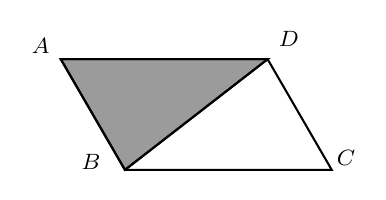
\begin{tikzpicture}[x=0.75pt,y=0.75pt,yscale=-1,xscale=1]
        %uncomment if require: \path (0,1525); %set diagram left start at 0, and has height of 1525
        %Shape: Polygon [id:ds07799279811843363] 
        \draw  [fill={rgb, 255:red, 155; green, 155; blue, 155 }  ,fill opacity=1 ] (509.1,1043.02) -- (440.36,1096.35) -- (409.45,1043.02) -- cycle ;
        %Shape: Parallelogram [id:dp08721857070673877] 
        \draw   (409.45,1043.02) -- (509.1,1043.02) -- (540,1096.35) -- (440.36,1096.35) -- cycle ;
        %Straight Lines [id:da9774868009248627] 
        \draw    (509.1,1043.02) -- (440.36,1096.35) ;
        % Text Node
        \draw (394,1031.35) node [anchor=north west][inner sep=0.75pt]  [font=\footnotesize]  {$A$};
        % Text Node
        \draw (418,1087.35) node [anchor=north west][inner sep=0.75pt]  [font=\footnotesize]  {$B$};
        % Text Node
        \draw (541,1085.35) node [anchor=north west][inner sep=0.75pt]  [font=\footnotesize]  {$C$};
        % Text Node
        \draw (513,1028.35) node [anchor=north west][inner sep=0.75pt]  [font=\footnotesize]  {$D$};
    \end{tikzpicture}
    \vspace{2em}
}
\marginnote{    对角线推论1:$ \triangle{ABD} \cong \triangle{BDC} $}


\begin{marginfigure}
    \includegraphics{1-area-4.jpg}
\end{marginfigure}
\marginnote{面积推论2:$ S_{\triangle{ABO}} = S_{\triangle{ADO}} = S_{\triangle{DOC}} = S_{\triangle{BOC}} $}


\begin{marginfigure}
    \includegraphics{1-area-2.jpg}
\end{marginfigure}
\marginnote{    过O直线推论3:$ \triangle AEO\ \cong \ \triangle CFO $}


\begin{marginfigure}
    \includegraphics{s1s2s3s4.png}
\end{marginfigure}
\marginnote{面积推论4:$ S_1 \times S_3= S_2 \times S_4 $}

\begin{marginfigure}
    \includegraphics{1-area-3.jpg}
\end{marginfigure}
\marginnote{过O直线推论5:$ S_{1} =S_{2} +S_{3} =\frac{1}{2} S_{\pllg ABCD} $}

\begin{marginfigure}
    \includegraphics{1-s1s2duijiao.png}
\end{marginfigure}
\marginnote{    面积推论6:$S_{1} +S_{2} =S_{3} +S_{4} =\frac{1}{2} S_{\pllg ABCD}$}








\begin{theorem}
    \textbf{平行四边形重要推论:对角线与过O直线---“4”}
    \begin{itemize}
        \item 结论:单对角线分两等---全等
        \item 结论:双对角线分四等---等面积
        \item 结论:过 O 直线与对角线成全等
        \item 结论:过 O 直线平分面积与周长       
    \end{itemize}
\end{theorem}

\begin{theorem}
    \textbf{平行四边形重要推论:关于面积---“3”}
    \begin{itemize}
        \item 结论:十字平行分   
        \item 结论:顶点对边分
        \item 结论:四顶点加一点分   
    \end{itemize}
\end{theorem}





\cleardoublepage












\cleardoublepage
\section{课堂随练}

本节的重点在于:“两条对边,一个对称中心,两条对角线”,理解\ubi{对边平行}是平四的核心性质, 
\ubi{对称中心}是平四最重要的几何中心(作图、面积题常用),\ubi{对角线}对于整个四边形的分割起核心作用(证明题常用)。



\subsection{基础:性质、角度、长度、面积、坐标}




\begin{example}

    如图所示,已知四边形ABCD,从⑴AB//DC;⑵AB=DC;⑶AD//BC;⑷AD=BC;⑸∠A=∠C;⑹∠B=∠D中取两
    个条件加以组合,能推出四边形ABCD是平行四边形的有哪几种情形?请写出具体组合。

    % png
    \tikzset{every picture/.style={line width=0.75pt}} %set default line width to 0.75pt        
    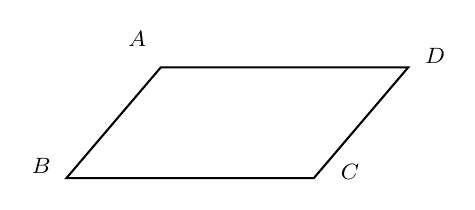
\begin{tikzpicture}[x=0.75pt,y=0.75pt,yscale=-1,xscale=1]
    %uncomment if require: \path (0,1741); %set diagram left start at 0, and has height of 1741
    %Shape: Parallelogram [id:dp3568520636381194] 
    \draw   (70.79,701.33) -- (190,701.33) -- (144.54,754.67) -- (25.33,754.67) -- cycle ;
    % Text Node
    \draw (53.72,682.67) node [anchor=north west][inner sep=0.75pt]  [font=\footnotesize]  {$A$};
    % Text Node
    \draw (7.19,743.67) node [anchor=north west][inner sep=0.75pt]  [font=\footnotesize]  {$B$};
    % Text Node
    \draw (156.05,746.67) node [anchor=north west][inner sep=0.75pt]  [font=\footnotesize]  {$C$};
    % Text Node
    \draw (196.73,690.67) node [anchor=north west][inner sep=0.75pt]  [font=\footnotesize]  {$D$};
    \end{tikzpicture}
\end{example}

\begin{answers}
    总共9种:① ⑴,⑶;② ⑵,⑷;③ ⑸,⑹;④ ⑴,⑵;
    ⑤ ⑶,⑷;⑥ ⑴,⑸;⑦ ⑴,⑹;⑧ ⑶,⑸;⑨ ⑶,⑹.
\end{answers}

\begin{examplespace}
    \vspace{4cm}
\end{examplespace}


\begin{example}有下列说法:\\
①平行四边形具有四边形的所有性质;\\
②平行四边形是中心对称图形;\\③平行四边形的任一条对角线可把平行四边形分成两个全等的三角形;\\④平行四
边形的两条对角线把平行四边形分成4个面积相等的小三角形.\\其中正确说法的序号是(    )\\
A.①②④	B.①③④	C.①②③	D.①②③④
\end{example}

\begin{answers}
    【答案】D
    【分析】本题考查平行四边形的性质,根据平行四边形的性质逐个判断即可得到答案.
    【详解】解:平行四边形具有四边形的所有性质,故①正确,
    平行四边形是中心对称图形,故②正确,
    平行四边形的任意一条对角线可把平行四边形分成两个全等的三角形,故③正确,
    平行四边形的两条对角线把平行四边形分成4个面积相等的小三角形,故④正确,
    故选:D.
\end{answers}



\example{}下面关于平行四边形的性质描述正确的是(  )\\
A.平行四边形的对称中心是对角线的交点\\
B.平行四边形的对称轴是对角线所在直线\\
C.平行四边形不是中心对称图形\\
D.平行四边形既不是中心对称图形,也不是轴对称图形






\example{}在平行四边形 ABCD 中,$\angle{B}-\angle{A}=20^o$ 则
$\angle{D}$的度数是?

\begin{examplespace}
    \vspace{2cm}
\end{examplespace}





\example{}如图,在平行四边形ABCD中,已知∠ODA=90°,AC=10cm ,BD=6cm ,则AD的长为(\ \ \ )\\
\tikzset{every picture/.style={line width=0.75pt}} %set default line width to 0.75pt        
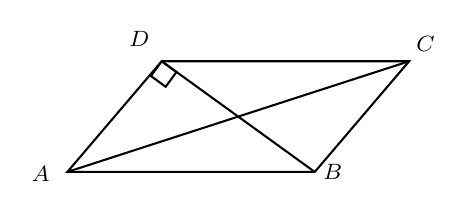
\begin{tikzpicture}[x=0.75pt,y=0.75pt,yscale=-1,xscale=1]
%uncomment if require: \path (0,862); %set diagram left start at 0, and has height of 862
%Shape: Parallelogram [id:dp5579947545995634] 
\draw   (81.79,456.47) -- (201,456.47) -- (155.54,509.8) -- (36.33,509.8) -- cycle ;
%Straight Lines [id:da08553774693266791] 
\draw    (36.33,509.8) -- (201,456.47) ;
%Straight Lines [id:da863825186807412] 
\draw    (155.54,509.8) -- (81.79,456.47) ;
%Shape: Square [id:dp6977752958600176] 
\draw   (81.79,456.47) -- (88.9,461.66) -- (83.71,468.77) -- (76.6,463.58) -- cycle ;
% Text Node
\draw (17.72,505.8) node [anchor=north west][inner sep=0.75pt]  [font=\footnotesize]  {$A$};
% Text Node
\draw (158.19,504.8) node [anchor=north west][inner sep=0.75pt]  [font=\footnotesize]  {$B$};
% Text Node
\draw (203.05,442.8) node [anchor=north west][inner sep=0.75pt]  [font=\footnotesize]  {$C$};
% Text Node
\draw (64.73,440.8) node [anchor=north west][inner sep=0.75pt]  [font=\footnotesize]  {$D$};
\end{tikzpicture}
\\
A. 4cm \ \ \ B. 5cm \ \ \  C. 6cm \ \ \  D. 8cm

\begin{answers}
    故答案为: A
\end{answers}

\begin{examplespace}
    \vspace{1cm}
\end{examplespace}




\example{} 在平行四边形ABCD中,AD=10,AE平分∠BAD交BC于点E,DF平分∠ADC交BC于点F,且EF=2,则AB的长为( \ )\\
A.4  \hspace{2em}	B.6 \hspace{2em} C.6或8 \hspace{2em} D.4或6

\begin{answers}
    当点F在点E的左侧时:BC=BE-EF+CF=2AB-EF=10,∴AB=6;\\
    当点F在点E的右侧时,BC=BE+EF+CF=2AB+EF=10,∴AB=4
\end{answers}

\begin{examplespace}
    \vspace{1cm}
\end{examplespace}

\begin{example}
    如图,在平行四边形ABCD中,P是AD边上一点.已知 $S_{△ABP}=3.5cm^2$,
    $S_{△CDP}=2.5cm^2$ ,则ABCD的面积是 \underline{\hspace{3em}}cm2.
\end{example}

\tikzset{every picture/.style={line width=0.75pt}} %set default line width to 0.75pt        
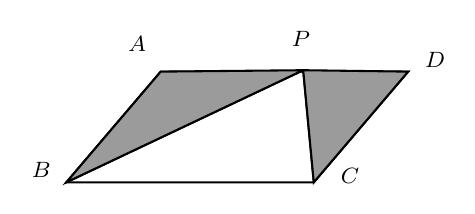
\begin{tikzpicture}[x=0.75pt,y=0.75pt,yscale=-1,xscale=1]
%uncomment if require: \path (0,862); %set diagram left start at 0, and has height of 862
%Shape: Parallelogram [id:dp5579947545995634] 
\draw   (142.79,377.47) -- (262,377.47) -- (216.54,430.8) -- (97.33,430.8) -- cycle ;
%Straight Lines [id:da08553774693266791] 
\draw    (97.33,430.8) -- (211.43,376.79) ;
%Straight Lines [id:da863825186807412] 
\draw    (216.54,430.8) -- (211.43,376.79) ;
%Shape: Polygon [id:ds8461736670609956] 
\draw  [fill={rgb, 255:red, 155; green, 155; blue, 155 }  ,fill opacity=1 ] (211.43,376.79) -- (142.79,377.47) -- (97.33,430.8) -- cycle ;
%Shape: Polygon [id:ds8484543599248031] 
\draw  [fill={rgb, 255:red, 155; green, 155; blue, 155 }  ,fill opacity=1 ] (211.43,376.79) -- (262,377.47) -- (216.54,430.8) -- cycle ;
% Text Node
\draw (125.72,358.8) node [anchor=north west][inner sep=0.75pt]  [font=\footnotesize]  {$A$};
% Text Node
\draw (79.19,419.8) node [anchor=north west][inner sep=0.75pt]  [font=\footnotesize]  {$B$};
% Text Node
\draw (228.05,422.8) node [anchor=north west][inner sep=0.75pt]  [font=\footnotesize]  {$C$};
% Text Node
\draw (268.73,366.8) node [anchor=north west][inner sep=0.75pt]  [font=\footnotesize]  {$D$};
% Text Node
\draw (204.52,356.8) node [anchor=north west][inner sep=0.75pt]  [font=\footnotesize]  {$P$};
\end{tikzpicture}

\begin{answers}
    故答案为: 12
\end{answers}

\begin{examplespace}
    \vspace{1cm}
\end{examplespace}

\begin{example}
如图,平行四边形ABCD的对角线AC,BD相交于点O,EF,GH过点O,且点E,H在边AB上,点G,F在边CD上,则阴影部分的面积与ABCD的面积比值是(  ).\\
A.1/2  \hspace{2em}	B. 1/3 \hspace{2em}	C.1/4	\hspace{2em} D.1/5
\end{example}

\tikzset{every picture/.style={line width=0.75pt}} %set default line width to 0.75pt        
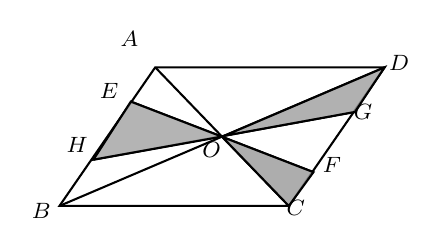
\begin{tikzpicture}[x=0.75pt,y=0.75pt,yscale=-1,xscale=1]
%uncomment if require: \path (0,862); %set diagram left start at 0, and has height of 862
%Shape: Parallelogram [id:dp06038619163205894] 
\draw   (90.2,565.72) -- (200.71,565.72) -- (154.56,632.51) -- (44.05,632.51) -- cycle ;
%Straight Lines [id:da3560331603396958] 
\draw    (44.04,632.51) -- (200.71,565.72) ;
%Straight Lines [id:da8763632420613607] 
\draw    (154.56,632.51) -- (90.2,565.72) ;
%Straight Lines [id:da2281992729302893] 
\draw    (166.43,616.22) -- (78.43,582.22) ;
%Straight Lines [id:da6079753294224146] 
\draw    (186.43,587.22) -- (60.43,610.22) ;
%Shape: Polygon [id:ds004984977602802809] 
\draw  [fill={rgb, 255:red, 155; green, 155; blue, 155 }  ,fill opacity=0.75 ] (60.43,610.22) -- (78.43,582.22) -- (122.38,599.11) -- cycle ;
%Shape: Polygon [id:ds9215486577189165] 
\draw  [fill={rgb, 255:red, 155; green, 155; blue, 155 }  ,fill opacity=0.78 ] (186.43,587.22) -- (200.71,565.72) -- (123.43,598.72) -- cycle ;
%Shape: Polygon [id:ds1137429846365201] 
\draw  [fill={rgb, 255:red, 155; green, 155; blue, 155 }  ,fill opacity=0.82 ] (154.56,632.51) -- (166.43,616.22) -- (122.43,599.22) -- cycle ;
% Text Node
\draw (71.97,547.12) node [anchor=north west][inner sep=0.75pt]  [font=\footnotesize]  {$A$};
% Text Node
\draw (29.24,629.77) node [anchor=north west][inner sep=0.75pt]  [font=\footnotesize]  {$B$};
% Text Node
\draw (152.05,628.52) node [anchor=north west][inner sep=0.75pt]  [font=\footnotesize]  {$C$};
% Text Node
\draw (201.44,558.39) node [anchor=north west][inner sep=0.75pt]  [font=\footnotesize]  {$D$};
% Text Node
\draw (61.99,571.87) node [anchor=north west][inner sep=0.75pt]  [font=\footnotesize]  {$E$};
% Text Node
\draw (169.5,607.79) node [anchor=north west][inner sep=0.75pt]  [font=\footnotesize]  {$F$};
% Text Node
\draw (45.99,597.87) node [anchor=north west][inner sep=0.75pt]  [font=\footnotesize]  {$H$};
% Text Node
\draw (184.43,582.22) node [anchor=north west][inner sep=0.75pt]  [font=\footnotesize]  {$G$};
% Text Node
\draw (111.43,600.22) node [anchor=north west][inner sep=0.75pt]  [font=\footnotesize]  {$O$};
\end{tikzpicture}

\begin{answers}
    阴影部分的面积与▱ABCD的面积比值是1/4.故选:C.
\end{answers}



\cleardoublepage

\begin{example}
    如图,在平面直角坐标系中,若平行四边形ABCD的三个顶点的坐标分别是A(-1,0)、B(-2,-3)、
    D(3,2),则顶点C的坐标是 \uds .
\end{example}

\tikzset{every picture/.style={line width=0.75pt}} %set default line width to 0.75pt        
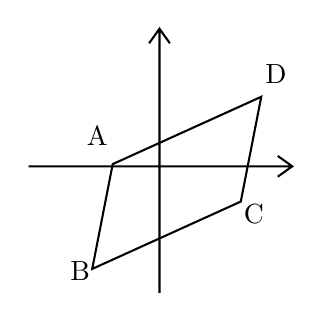
\begin{tikzpicture}[x=0.75pt,y=0.75pt,yscale=-1,xscale=1]
%uncomment if require: \path (0,939); %set diagram left start at 0, and has height of 939
%Shape: Axis 2D [id:dp5911960483097314] 
\draw  (49.43,772.08) -- (176.43,772.08)(112.43,705.79) -- (112.43,833.08) (169.43,767.08) -- (176.43,772.08) -- (169.43,777.08) (107.43,712.79) -- (112.43,705.79) -- (117.43,712.79)  ;
%Shape: Parallelogram [id:dp41646868203937903] 
\draw   (89.9,771.01) -- (161.47,738.58) -- (151.6,789.07) -- (80.03,821.51) -- cycle ;
% Text Node
\draw (162,721.65) node [anchor=north west][inner sep=0.75pt]   [align=left] {D};
% Text Node
\draw (76,751.65) node [anchor=north west][inner sep=0.75pt]   [align=left] {A};
% Text Node
\draw (68,816.65) node [anchor=north west][inner sep=0.75pt]   [align=left] {B};
% Text Node
\draw (151.6,789.07) node [anchor=north west][inner sep=0.75pt]   [align=left] {C};
\end{tikzpicture}

\begin{answers}
    故答案为: (2,-1).
\end{answers}   



\example{}以三角形的三个顶点作平行四边形,最多可以作( \ \ )\\
A.2个     \ \  B.3个  \ \      C.4个  \ \       D.5个

% -------
% 平行四边形存在性问题引入
% -------   
\marginnote{
    【探索】请你尝试利用下图坐标系,画出符合要求的平行四边形。【注意】这个问题叫平四
    存在性问题,是八下其中的常考内容,题目会要求你回答能与已知三点构成平四的第四个点
    的坐标。
}
\begin{marginfigure}
    \includegraphics{1-cordi-pllg.png}
\end{marginfigure}

\begin{answers}
    答案 B,3个
\end{answers}

\begin{examplespace}
    \vspace{7cm}
\end{examplespace}







\subsection{提高:性质相关证明问题}

\begin{example}
    如图,平行四边形ABCD的对角线AC,BD交于点O,AE平分∠BAD,交BC于点E,且∠ADC=60°,
    $AB=\frac{1}{2}BC$,    连接OE,下列结论\\①∠CAD=30°;\\②OE⊥AC;\\③$BD=\sqrt{7}AB$;\\
    ④$S_{\pllg ABOE}=\frac{3}{2}S_{△OCD}$;\\其中成立的个数是(  \ \  )\\
     A.1个	 \ \   B.2个  \ \    C.3个  \ \   D.4个

     \tikzset{every picture/.style={line width=0.75pt}} %set default line width to 0.75pt        
     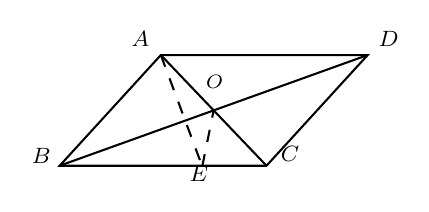
\begin{tikzpicture}[x=0.75pt,y=0.75pt,yscale=-1,xscale=1]
     %uncomment if require: \path (0,1636); %set diagram left start at 0, and has height of 1636
     %Shape: Parallelogram [id:dp7805901493252498] 
     \draw   (526.38,1092.02) -- (626.02,1092.02) -- (577.28,1145.35) -- (477.64,1145.35) -- cycle ;
     %Straight Lines [id:da11225844031236476] 
     \draw    (526.38,1092.02) -- (577.28,1145.35) ;
     %Straight Lines [id:da12493476484801858] 
     \draw    (626.02,1092.02) -- (477.64,1145.35) ;
     %Straight Lines [id:da9626816487519783] 
     \draw  [dash pattern={on 4.5pt off 4.5pt}]  (526.38,1092.02) -- (546.33,1145.69) ;
     %Straight Lines [id:da7534701376090551] 
     \draw  [dash pattern={on 4.5pt off 4.5pt}]  (546.33,1145.69) -- (551.83,1118.69) ;
     % Text Node
     \draw (510.84,1079.35) node [anchor=north west][inner sep=0.75pt]  [font=\footnotesize]  {$A$};
     % Text Node
     \draw (462.72,1135.35) node [anchor=north west][inner sep=0.75pt]  [font=\footnotesize]  {$B$};
     % Text Node
     \draw (582.71,1134.35) node [anchor=north west][inner sep=0.75pt]  [font=\footnotesize]  {$C$};
     % Text Node
     \draw (629.83,1079.35) node [anchor=north west][inner sep=0.75pt]  [font=\footnotesize]  {$D$};
     % Text Node
     \draw (546.63,1100.35) node [anchor=north west][inner sep=0.75pt]  [font=\scriptsize]  {$O$};
     % Text Node
     \draw (538.71,1144.35) node [anchor=north west][inner sep=0.75pt]  [font=\footnotesize]  {$E$};
     \end{tikzpicture}
\end{example}

\begin{answers}
    D
    【分析】结合平行四边形的性质可证明△ABE为等边三角形,由BC=AD=2AB,可判断①,
    由EC=AE,AO=CO,得OE⊥AC,故②正确,设 ,则BC=2x,对"Rt"△BAC,"Rt"△ABO运用勾
    股定理即可判断③,利用三角形中线的性质结合三角形的面积可求解判断④.
\end{answers}   

\begin{examplespace}
    \vspace{3cm}
\end{examplespace}

\subsection{提高:绘图专题}
\begin{example}
    \sidenote{
        【提示】
        \begin{itemize}
            \item 过圆心的直线总是平分圆的周长和面积, 实际上任何一个中心对称图形都有这个性质:过对称中心的
            直线,平分周长和面积。
            \item 想想如果一条线要同时平分两个中心对称图形的面积和周长,该怎么办?
        \end{itemize}    
    }
    在一块平行四边形的稻田里有一圆形的水池,为了给稻田浇水,并使稻田里的
    水量趋于均匀,现要从水池引一条笔直的水渠(水渠的宽度忽略不计),
    请你设计一种方案,使水渠两侧的稻田面积相等,并说明你的理由.\\ \\

    \tikzset{every picture/.style={line width=0.75pt}} %set default line width to 0.75pt        
    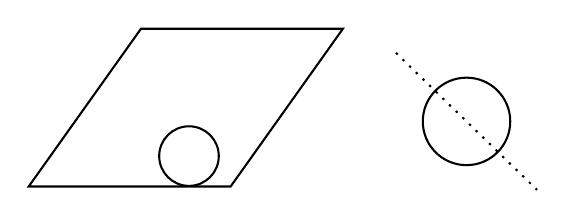
\begin{tikzpicture}[x=0.75pt,y=0.75pt,yscale=-1,xscale=1]
    %uncomment if require: \path (0,939); %set diagram left start at 0, and has height of 939
    %Shape: Parallelogram [id:dp21965265876855633] 
    \draw   (310.23,765.65) -- (407.52,765.65) -- (353.43,841.65) -- (256.14,841.65) -- cycle ;
    %Shape: Circle [id:dp05139693308100379] 
    \draw   (319,827.01) .. controls (319,819.08) and (325.43,812.65) .. (333.36,812.65) .. controls (341.29,812.65) and (347.71,819.08) .. (347.71,827.01) .. controls (347.71,834.94) and (341.29,841.37) .. (333.36,841.37) .. controls (325.43,841.37) and (319,834.94) .. (319,827.01) -- cycle ;
    %Shape: Circle [id:dp8600513021489369] 
    \draw   (446,810.29) .. controls (446,798.66) and (455.43,789.22) .. (467.07,789.22) .. controls (478.71,789.22) and (488.14,798.66) .. (488.14,810.29) .. controls (488.14,821.93) and (478.71,831.37) .. (467.07,831.37) .. controls (455.43,831.37) and (446,821.93) .. (446,810.29) -- cycle ;
    %Straight Lines [id:da2613202665852332] 
    \draw  [dash pattern={on 0.84pt off 2.51pt}]  (433.07,777.29) -- (501.07,843.29) ;
    \end{tikzpicture}
\end{example}



\begin{example}
    \sidenote{
        【提示】
        \begin{itemize}
            \item 平四作图最常用的就是“对称中心”,经常构造新的中心对称图形解决问题
            \item 如何找对称中心就是需要考虑的第一步,第二步是如何构造中心对称图形
            \item 对于“找点”,两线交一点;对于“找线”,两点定一线。
        \end{itemize}
    }
    已知平行四边形ABCD是中心对称图形,点E是平面上一点,请仅用无
    刻度直尺画出点E关于ABCD对称中心的对称点F.\\
    (1)如图1,点E在ABCD的边AD上;\\
    (2)如图2,点E在ABCD外.\\

    \tikzset{every picture/.style={line width=0.75pt}} %set default line width to 0.75pt        
    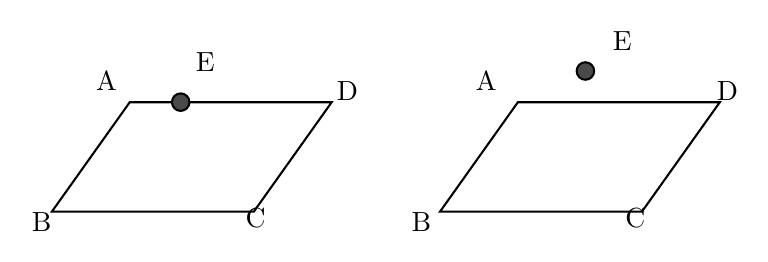
\begin{tikzpicture}[x=0.75pt,y=0.75pt,yscale=-1,xscale=1]
    %uncomment if require: \path (0,1083); %set diagram left start at 0, and has height of 1083
    %Shape: Parallelogram [id:dp8038026768378546] 
    \draw   (132.66,934.22) -- (229.95,934.22) -- (192.43,986.94) -- (95.14,986.94) -- cycle ;
    %Shape: Parallelogram [id:dp5462257042242362] 
    \draw   (319.66,934.22) -- (416.95,934.22) -- (379.43,986.94) -- (282.14,986.94) -- cycle ;
    %Shape: Circle [id:dp18747520040402943] 
    \draw  [fill={rgb, 255:red, 74; green, 74; blue, 74 }  ,fill opacity=1 ] (153,934.15) .. controls (153,931.82) and (154.89,929.94) .. (157.21,929.94) .. controls (159.54,929.94) and (161.43,931.82) .. (161.43,934.15) .. controls (161.43,936.48) and (159.54,938.37) .. (157.21,938.37) .. controls (154.89,938.37) and (153,936.48) .. (153,934.15) -- cycle ;
    %Shape: Circle [id:dp19840861894910566] 
    \draw  [fill={rgb, 255:red, 74; green, 74; blue, 74 }  ,fill opacity=1 ] (348,919.15) .. controls (348,916.82) and (349.89,914.94) .. (352.21,914.94) .. controls (354.54,914.94) and (356.43,916.82) .. (356.43,919.15) .. controls (356.43,921.48) and (354.54,923.37) .. (352.21,923.37) .. controls (349.89,923.37) and (348,921.48) .. (348,919.15) -- cycle ;
    % Text Node
    \draw (115,917.79) node [anchor=north west][inner sep=0.75pt]   [align=left] {A};
    % Text Node
    \draw (84,985.79) node [anchor=north west][inner sep=0.75pt]   [align=left] {B};
    % Text Node
    \draw (187,983.79) node [anchor=north west][inner sep=0.75pt]   [align=left] {C};
    % Text Node
    \draw (231,922.79) node [anchor=north west][inner sep=0.75pt]   [align=left] {D};
    % Text Node
    \draw (298,917.79) node [anchor=north west][inner sep=0.75pt]   [align=left] {A};
    % Text Node
    \draw (267,985.79) node [anchor=north west][inner sep=0.75pt]   [align=left] {B};
    % Text Node
    \draw (370,983.79) node [anchor=north west][inner sep=0.75pt]   [align=left] {C};
    % Text Node
    \draw (414,922.79) node [anchor=north west][inner sep=0.75pt]   [align=left] {D};
    % Text Node
    \draw (163,908.79) node [anchor=north west][inner sep=0.75pt]   [align=left] {E};
    % Text Node
    \draw (364,898.79) node [anchor=north west][inner sep=0.75pt]   [align=left] {E};
    \end{tikzpicture}
\end{example}


\cleardoublepage




\subsection{提高:动点问题}
\begin{example}
    如图,在平行四边形ABCD中,∠BAC=90°,∠B=60°,AB=6.动点P从点A出发沿AD以1cm/s速度向终
    点D运动,同时点Q从点C出发,以4cm/s速度沿射线CB运动,当点P到达终点时,点Q也随之停止运
    动,设点P运动的时间为t秒.\\
    (1)用含t的代数式表示BQ= \uds ;\\
    (2)当PQ⊥BC时, 求t的值;\\
    (3)请问是否存在t的值,使得A,B,P,Q为顶点的四边形为平行四边形? 若存在,求出t的
    值;若不存在,请说明理由.

    \includegraphics{images/dongdian-t1.jpg}
\end{example}

\begin{answers}
    (1)BQ=12-4t(0≤t≤3)或BQ=4t-12(3<t≤12)
    (2)9/5, AP=QH, t=9-4t, t=9/5
    (3)存在,12/5或4, (1)当AB为边时,AP=BQ, t=12-4t,四边形ABQP是平行四边形,(2)当AB为对角线时,AP=BQ, 
    ,t=4t-12, 四边形 APBQ 是平四。
\end{answers}    





\cleardoublepage
\section{课堂内容回忆}

\ubi{姓名:} \uds\uds \ \ \ \ \ubi{日期:} \uds\uds

\begin{exercise} 课堂回忆
    \begin{enumerate}
    \item 我们一开始回忆了八上的什么概念\uds\uds, 他的定义是什么?
    \uds \uds \uds.
    \item 他与我们今天学习的内容有什么区别,今天学习的对称叫什么,定义是什么
    \uds \uds \uds. 
\end{enumerate}
\end{exercise}


\begin{exercise} 课堂回忆
    \begin{enumerate} 
    \item 已知轴对称图形上的点坐标(a,b)及其对应点(m,n),能否求出对称轴的表达式
    \uds \uds
    \item  已知中心对称图形上的点坐标 (a,b) 及其对应点 (m,n)能否求出对称中心的坐标
    \uds \uds
\end{enumerate}
\end{exercise}


\begin{exercise} 课堂回忆\\
    如何绘制轴对称图形,以及中心对称图形。以一条线段为例进行说明(请绘制出坐标系、及任意一条线段并绘图说明)。
\end{exercise}

\begin{exercise} 课堂回忆
    \begin{enumerate}
    \item 平行四边形的定义什么?\uds \uds \uds
    \item 平行四边形的性质,可以归结为两个核心性质,他们是 \uds \uds 和 \uds \uds
    \item 其中 “两组对边分别平行” 可以推出 :\\
        (1) \uds \uds
        (2) \uds \uds
        (3) \uds \uds 
    \end{enumerate}
\end{exercise}

\begin{exercise} 课堂回忆\\
    关于平四的“4+3”个重要推论(请绘图说明):
\end{exercise}






\cleardoublepage
\section{课后作业}
\exercise{} 平行四边形具有而一般四边形不具有的性质是(    )
A.外角和等于	\\
B.对角线互相平分\\
C.内角和等于	\\
D.有两条对角线\\

\exercise{}如图,在平行四边形 ABCD 中,$\angle{D}=100^o$,\angle{DAB}的平
分线AE交CD于点E,连接BE, 若$AE=AB$,则\angle{EBC}的度数为\underline{\hspace{2em}}.

\tikzset{every picture/.style={line width=0.75pt}} %set default line width to 0.75pt        
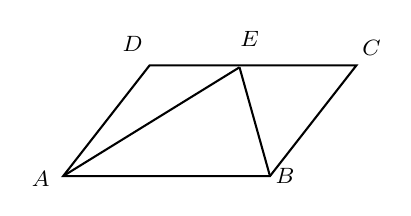
\begin{tikzpicture}[x=0.75pt,y=0.75pt,yscale=-1,xscale=1]
%uncomment if require: \path (0,862); %set diagram left start at 0, and has height of 862
%Shape: Parallelogram [id:dp5579947545995634] 
\draw   (127.87,631.47) -- (227.51,631.47) -- (185.88,684.8) -- (86.24,684.8) -- cycle ;
%Straight Lines [id:da08553774693266791] 
\draw    (86.24,684.8) -- (171.2,632.38) ;
%Straight Lines [id:da863825186807412] 
\draw    (185.88,684.8) -- (171.2,632.38) ;
% Text Node
\draw (69.64,680.8) node [anchor=north west][inner sep=0.75pt]  [font=\footnotesize]  {$A$};
% Text Node
\draw (187.12,679.8) node [anchor=north west][inner sep=0.75pt]  [font=\footnotesize]  {$B$};
% Text Node
\draw (228.84,617.8) node [anchor=north west][inner sep=0.75pt]  [font=\footnotesize]  {$C$};
% Text Node
\draw (113.36,615.8) node [anchor=north west][inner sep=0.75pt]  [font=\footnotesize]  {$D$};
% Text Node
\draw (170.16,613.8) node [anchor=north west][inner sep=0.75pt]  [font=\footnotesize]  {$E$};
\end{tikzpicture}

\begin{answers}
    故答案为: 30度
\end{answers}


\exercise{}如图,四边形ABCD是平行四边形,∠ABC=70°, BE平分∠ABC且交AD于点E,DF//BE
且交BC于点F,则∠ADF的度数为\underline{\hspace{3em}}.

\tikzset{every picture/.style={line width=0.75pt}} %set default line width to 0.75pt        
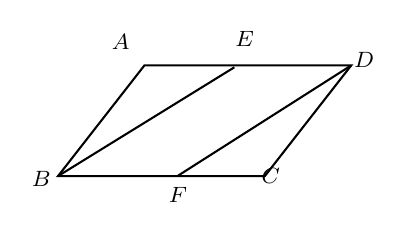
\begin{tikzpicture}[x=0.75pt,y=0.75pt,yscale=-1,xscale=1]
%uncomment if require: \path (0,862); %set diagram left start at 0, and has height of 862
%Shape: Parallelogram [id:dp06038619163205894] 
\draw   (84.23,584.47) -- (183.87,584.47) -- (142.24,637.8) -- (42.6,637.8) -- cycle ;
%Straight Lines [id:da3560331603396958] 
\draw    (42.6,637.8) -- (127.56,585.38) ;
%Straight Lines [id:da8763632420613607] 
\draw    (100.43,637.6) -- (183.87,584.47) ;
% Text No
\draw (67,567.8) node [anchor=north west][inner sep=0.75pt]  [font=\footnotesize]  {$A$};
% Text Node
\draw (28.48,633.8) node [anchor=north west][inner sep=0.75pt]  [font=\footnotesize]  {$B$};
% Text Node
\draw (139.2,632.8) node [anchor=north west][inner sep=0.75pt]  [font=\footnotesize]  {$C$};
% Text Node
\draw (183.72,576.8) node [anchor=north west][inner sep=0.75pt]  [font=\footnotesize]  {$D$};
% Text Node
\draw (126.52,566.8) node [anchor=north west][inner sep=0.75pt]  [font=\footnotesize]  {$E$};
% Text Node
\draw (94.52,641.8) node [anchor=north west][inner sep=0.75pt]  [font=\footnotesize]  {$F$};
\end{tikzpicture}

\begin{exercise}
    如图,四边形 ABCD 是平行四边形.若 $S_{ABCD}=12$, 则 $S_\text{阴影}=\uds$.\\
    \includegraphics[width=0.5\textwidth]{1-area-1.png}
\end{exercise}

\begin{answers}
        阴影面积=3
\end{answers}


\exercise{}在平面直角坐标系里,A(1,0),B(0,2),C(-4,2),若以A、B、C、D为顶点的四边形是平
行四边形,则点D的坐标为\uds.

\begin{examplespace}
    \vspace{2cm}
\end{examplespace}


\cleardoublepage
\begin{exercise}
    在平行四边形ABCD中,对角线AC,BD相交于点O,以点O为坐标原点建立平面直角坐标系,
    其中A(a,b),B(a-1,b+2),C(3,1),则点D的坐标是\underline{\hspace{3em}}.
\end{exercise}

\begin{answers}
    故答案为: (4,-1)
\end{answers}

\begin{examplespace}
    \vspace{2cm}
\end{examplespace}





\begin{exercise}
    $$
    \begin{aligned}
        &\text{如图,在平面直角坐标系中},A(1,1),B(2,-1),\text{且以A,B,O,C 为顶点的四边形为平行四}\\& \text{边形,则点C的坐标为}\uds
    \end{aligned}
    $$
    \includegraphics[width=0.5\textwidth]{1-corrdinate.png}
\end{exercise}



\begin{exercise}
    如图,在平行四边形ABCD中,对角线AC,BD交于点O,AB=2, ,$∠ABC=60^∘$,直线EF过
    点O,连接DF,交AC于点G,连BG,△DCF的周长等于6,下列说法正确的个数为(  \  )
    \\①$ ∠EOD=90^∘ $;\\② $S_{△DFC} = 2S_{△AEO}$ \\
    ③ $ S_{△ABG}+S_{△DGC} =\frac{1}{2} S_{\pllg ABCD} $;
    \\④ $ AE=\frac{6}{5} $.
 
    A.1个	\ B.2个\ 	C.3个	\ D.4个

    \tikzset{every picture/.style={line width=0.75pt}} %set default line width to 0.75pt        
    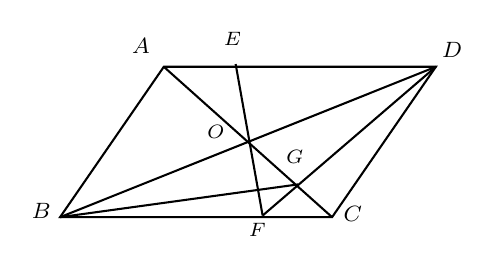
\begin{tikzpicture}[x=0.75pt,y=0.75pt,yscale=-1,xscale=1]
    %uncomment if require: \path (0,1954); %set diagram left start at 0, and has height of 1954
    %Shape: Parallelogram [id:dp5445386943379376] 
    \draw   (109.72,1032.66) -- (240.78,1032.66) -- (190.8,1105.11) -- (59.74,1105.11) -- cycle ;
    %Straight Lines [id:da7725624291564848] 
    \draw    (157.33,1104.34) -- (144.33,1031.34) ;
    %Straight Lines [id:da679340776586659] 
    \draw    (109.72,1032.66) -- (190.8,1105.11) ;
    %Straight Lines [id:da3761082926784409] 
    \draw    (59.74,1105.11) -- (240.78,1032.66) ;
    %Straight Lines [id:da7134684897107266] 
    \draw    (157.33,1104.34) -- (240.78,1032.66) ;
    %Straight Lines [id:da33257673335666316] 
    \draw    (174.33,1089.34) -- (59.74,1105.11) ;
    % Text Node
    \draw (92.95,1017.53) node [anchor=north west][inner sep=0.75pt]  [font=\footnotesize]  {$A$};
    % Text Node
    \draw (44.63,1097.11) node [anchor=north west][inner sep=0.75pt]  [font=\footnotesize]  {$B$};
    % Text Node
    \draw (194.86,1098.47) node [anchor=north west][inner sep=0.75pt]  [font=\footnotesize]  {$C$};
    % Text Node
    \draw (242.26,1019.4) node [anchor=north west][inner sep=0.75pt]  [font=\footnotesize]  {$D$};
    % Text Node
    \draw (137.15,1014.33) node [anchor=north west][inner sep=0.75pt]  [font=\scriptsize]  {$E$};
    % Text Node
    \draw (167.15,1071.33) node [anchor=north west][inner sep=0.75pt]  [font=\scriptsize]  {$G$};
    % Text Node
    \draw (129.15,1059.33) node [anchor=north west][inner sep=0.75pt]  [font=\scriptsize]  {$O$};
    % Text Node
    \draw (149.15,1106.33) node [anchor=north west][inner sep=0.75pt]  [font=\scriptsize]  {$F$};
    \end{tikzpicture}
\end{exercise}

\begin{examplespace}
    \vspace{3cm}
\end{examplespace}


\begin{exercise}
    如图,E是 \pllg ABCD内一点,ED⊥CD,EB⊥BC,∠AED=135°,连接 ,AC,BD,下列结
    论:\\①∠ADE=∠ABE;\\②△BCE为等腰直角三角形; \\③$ DE+AB=\sqrt{2}BD $;\\④ $AE^2+AB^2=AC^2 $,
    \\其中正确的个数有 (  \  )\\
    A.1 个	 \ \ B.2 个	\ \ C.3 个	\ \ D.4 个

    \tikzset{every picture/.style={line width=0.75pt}} %set default line width to 0.75pt        
    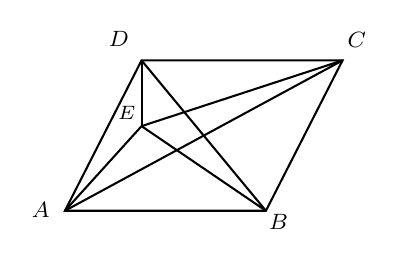
\begin{tikzpicture}[x=0.75pt,y=0.75pt,yscale=-1,xscale=1]
    %uncomment if require: \path (0,1954); %set diagram left start at 0, and has height of 1954
    %Shape: Parallelogram [id:dp0914658837696507] 
    \draw   (101.85,861.66) -- (198.68,861.66) -- (161.76,934.11) -- (64.93,934.11) -- cycle ;
    %Straight Lines [id:da10522305593889225] 
    \draw    (101.85,861.66) -- (101.85,893.33) ;
    %Straight Lines [id:da2586344429533527] 
    \draw    (64.93,934.11) -- (101.85,893.33) ;
    %Straight Lines [id:da6918464985413655] 
    \draw    (101.85,861.66) -- (161.76,934.11) ;
    %Straight Lines [id:da9211828674028979] 
    \draw    (64.93,934.11) -- (198.68,861.66) ;
    %Straight Lines [id:da33579659644280735] 
    \draw    (101.85,893.33) -- (198.68,861.66) ;
    %Straight Lines [id:da029590750307863622] 
    \draw    (101.85,893.33) -- (161.76,934.11) ;
    % Text Node
    \draw (47.48,928.53) node [anchor=north west][inner sep=0.75pt]  [font=\footnotesize]  {$A$};
    % Text Node
    \draw (161.76,934.11) node [anchor=north west][inner sep=0.75pt]  [font=\footnotesize]  {$B$};
    % Text Node
    \draw (199.61,846.47) node [anchor=north west][inner sep=0.75pt]  [font=\footnotesize]  {$C$};
    % Text Node
    \draw (84.65,846.4) node [anchor=north west][inner sep=0.75pt]  [font=\footnotesize]  {$D$};
    % Text Node
    \draw (89,882.33) node [anchor=north west][inner sep=0.75pt]  [font=\scriptsize]  {$E$};
    \end{tikzpicture}
\end{exercise}

\begin{answers}
    【答案】C
    【分析】①延长DE交AB于点F,根据平行四边形性质和四边形内角和即可得
    到∠ADE=∠ABE;②先证明△ADF≌△EBF,得AD=BE,又有AD=BC,可得BE=BC,即可得到
    △BCE为等腰直角三角形;③过点B作 交DC延长线于点G,证明△BDE≌△BCG,再根据勾
    股定理及等腰直角三角形的性质,可得DE+AB=√2 BD成立;④过点C作CH⊥AB于 ,根据勾股定
    理即可证明 $AC^2=AH^2+CH^2=(AB+√2/2 AE)^2+(AB-√2/2 AE)^2=2AB^2+AE^2$,可知结论不成立.
\end{answers}

\begin{examplespace}
    \vspace{1cm}
\end{examplespace}


\begin{exercise}仅用无刻度直尺作图:
    \begin{enumerate}[label=(\arabic*)]
        \item 如图1, 点 A, B, C, D 均在格点上, 在 AC 上找点 E, 使DE//AB;
        \item 如图2, 点 A, B, C 均在格点上, 作平行四边形 ABCD, 再在 CD 上作点 N , 使 CN = AM;
        \item 如图3, 过点 C 作 CD ⟂ AB;
        \item 如图4, 作点EF=$\sqrt{10}$(每个小正方形的边长为1).
    \end{enumerate}

    \includegraphics{1-draw3.png}
\end{exercise}

\begin{answers}
    \includegraphics{1-draw3-ans.png}
\end{answers}



\begin{exercise}
    $$
    \begin{aligned}
        &\text{如图 }1,\pllg ABCD,O\text{ 为 }AB\text{ 中点,过点 }B\text{ 作 }AC\text{ 的平行线}.\\
        &\text{变式}.\text{依照上述方法},\text{如图 }2,3,\text{点 }A,B\text{ 在格点上},\text{点 }C\text{ 在格线上},\text{过点 }C\text{ 作}\\
        &CD//AB.
    \end{aligned}
    $$

    \includegraphics{1-draw4.png}
\end{exercise}


\begin{answers}
    \includegraphics{1-draw4-ans.png}
\end{answers}

